\titledquestion{Neural Transition-Based Dependency Parsing}[54]

In this section, you'll be implementing a neural-network based dependency parser with the goal of maximizing performance on the UAS (Unlabeled Attachment Score) metric.\newline

Before you begin, please follow the README to install all the needed dependencies for the assignment. We will be using PyTorch 2.1.2 from \url{https://pytorch.org/get-started/locally/} with the \texttt{CUDA} option set to \texttt{None}, and the tqdm package -- which produces progress bar visualizations throughout your training process. The official PyTorch website is a great resource that includes tutorials for understanding PyTorch's Tensor library and neural networks. \newline

A dependency parser analyzes the grammatical structure of a sentence, establishing relationships between \textit{head} words, and words which modify those heads. There are multiple types of dependency parsers, including transition-based parsers, graph-based parsers, and feature-based parsers. Your implementation will be a {\it transition-based} parser, which incrementally builds up a parse one step at a time. At every step it maintains a \textit{partial parse}, which is represented as follows:
\begin{itemize}
\item A {\it stack} of words that are currently being processed.
\item A {\it buffer} of words yet to be processed.
\item A list of {\it dependencies} predicted by the parser.
\end{itemize}
Initially, the stack only contains ROOT, the dependencies list is empty, and the buffer contains all words of the sentence in order. At each step, the parser applies a {\it transition} to the partial parse until its buffer is empty and the stack size is 1. The following transitions can be applied:
\begin{itemize}
\item \texttt{SHIFT}: removes the first word from the buffer and pushes it onto the stack.
\item \texttt{LEFT-ARC}: marks the second (second most recently added) item on the stack as a dependent of the first item and removes the second item from the stack, adding a \textit{first\_word} $\rightarrow$ \textit{second\_word} dependency to the dependency list.
\item \texttt{RIGHT-ARC}: marks the first (most recently added) item on the stack as a dependent of the second item and removes the first item from the stack, adding a \textit{second\_word} $\rightarrow$ \textit{first\_word} dependency to the dependency list.
\end{itemize}
On each step, your parser will decide among the three transitions using a neural network classifier.

\begin{parts}
    
    \part[4] \textcolor{black}{Go through the sequence of transitions needed for parsing the sentence {\it ``I presented my findings at the NLP conference''}. The dependency tree for the sentence is shown below. At each step, give the configuration of the stack and buffer, as well as what transition was applied this step and what new dependency was added (if any). The first three steps are provided below as an example.} \\

    %\begin{center}
    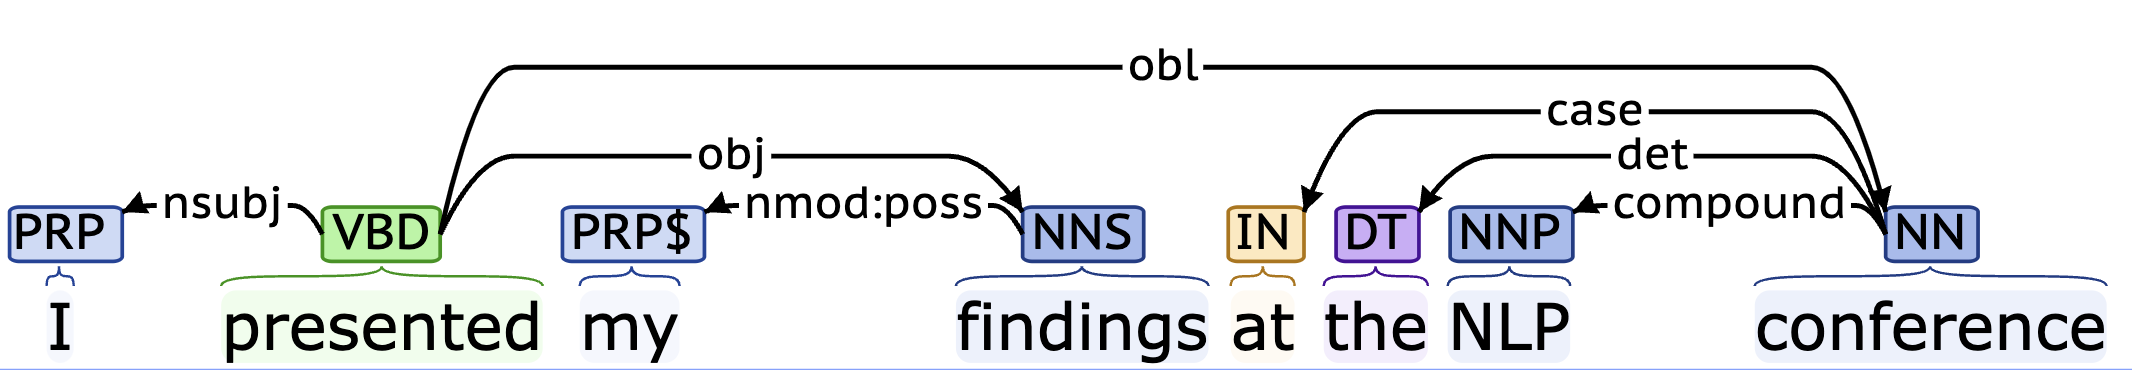
\includegraphics[width=0.8\textwidth]{example.png} \\
    %\end{center}

    \begin{adjustwidth}{-2cm}{}
    \begin{tabular}{ l | l | l | l}
    Stack & Buffer & New dependency & Transition \\ \hline
    [ROOT] & [I, presented, my, findings, at, the, NLP, conference] &  & Initial Configuration \\
    $[$ROOT, I] & [presented, my, findings, at, the, NLP, conference] &  &  \texttt{SHIFT}  \\
    $[$ROOT, I, presented] & [my, findings, at, the, NLP, conference] &  &  \texttt{SHIFT}  \\
    $[$ROOT, presented] & [my, findings, at, the, NLP, conference] & presented$\to$I &  \texttt{LEFT-ARC}  \\
    \end{tabular}\newline
    \end{adjustwidth}

\ifans{
\newline
\resizebox{\textwidth}{!}{%
    \begin{tabular}{ l | l | l | l}
    Stack & Buffer & New dependency & Transition \\ \hline
    [ROOT] & [I, presented, my, findings, at, the, NLP, conference] &  & Initial Configuration \\
    $[$ROOT, I] & [presented, my, findings, at, the, NLP, conference] &  &  \texttt{SHIFT}  \\
    $[$ROOT, I, presented] & [my, findings, at, the, NLP, conference] &  &  \texttt{SHIFT}  \\
    $[$ROOT, presented] & [my, findings, at, the, NLP, conference] & presented$\to$I &  \texttt{LEFT-ARC}  \\
    $[$ROOT, presented, my] & [findings, at, the, NLP, conference] &  &  \texttt{SHIFT} \\
    $[$ROOT, presented, my, findings] & [at, the, NLP, conference] &  &  \texttt{SHIFT} \\
    $[$ROOT, presented, findings] & [at, the, NLP, conference] & findings$\to$my  &  \texttt{LEFT-ARC} \\
    $[$ROOT, presented] & [at, the, NLP, conference] & presented$\to$findings  &  \texttt{RIGHT-ARC} \\
    $[$ROOT, presented, at] & [the, NLP, conference] &  &  \texttt{SHIFT} \\
    $[$ROOT, presented, at, the] & [NLP, conference] &  &  \texttt{SHIFT} \\
    $[$ROOT, presented, at, the, NLP] & [conference] &  &  \texttt{SHIFT} \\
    $[$ROOT, presented, at, the, NLP, conference] & [] &  &  \texttt{SHIFT} \\
    $[$ROOT, presented, at, the, conference] & [] & conference$\to$NLP &  \texttt{LEFT-ARC} \\
    $[$ROOT, presented, at, conference] & [] & conference$\to$the &  \texttt{LEFT-ARC} \\
    $[$ROOT, presented, conference] & [] & conference$\to$at &  \texttt{LEFT-ARC} \\
    $[$ROOT, presented] & [] & presented$\to$conference &  \texttt{RIGHT-ARC} \\
    $[$ROOT] & [] & ROOT$\to$presented &  \texttt{LEFT-ARC} \\
    \end{tabular}}
}
    
    \part[2] A sentence containing $n$ words will be parsed in how many steps (in terms of $n$)? Briefly explain in 1--2 sentences why.

\ifans{
We will need $2*n$ steps. For each word we need one operation to move the word from the buffer to the stack and another operation to create the relationship that removes the word from the stack.
}
    
    \part[6] Implement the \texttt{\_\_init\_\_} and \texttt{parse\_step} functions in the \texttt{PartialParse} class in \texttt{parser\_transitions.py}. This implements the transition mechanics your parser will use. You can run basic (non-exhaustive) tests by running \texttt{python parser\_transitions.py part\_c}.

    \part[8] Our network will predict which transition should be applied next to a partial parse. We could use it to parse a single sentence by applying predicted transitions until the parse is complete. However, neural networks run much more efficiently when making predictions about \textit{batches} of data at a time (i.e., predicting the next transition for any different partial parses simultaneously). We can parse sentences in minibatches with the following algorithm. \newline

    \alglanguage{pseudocode}
    \begin{algorithm*}[h]
    \caption{Minibatch Dependency Parsing}
    \begin{algorithmic}
    	\State \textbf{Input:} \texttt{sentences}, a list of sentences to be parsed and \texttt{model}, our model that makes parse decisions
    	%\State
    	%\State Initialize \texttt{partial\_parses} $\to$ []
    	%\For{\textbf{each} sentence \texttt{s} in \texttt{sentences}}
    	%	\State Add a partial parse to \texttt{partial\_parses} with \texttt{stack} = [ROOT], \texttt{buffer} = \texttt{s}, \texttt{dependencies} = []
    	%\EndFor
    	\State
    	\State Initialize \texttt{partial\_parses} as a list of PartialParses, one for each sentence in \texttt{sentences}
    	\State Initialize \texttt{unfinished\_parses} as a shallow copy of \texttt{partial\_parses}
    	%\State
    	\While{\texttt{unfinished\_parses} is not empty}

    		\State Take the first \texttt{batch\_size} parses in \texttt{unfinished\_parses} as a minibatch
    		\State Use the \texttt{model} to predict the next transition for each partial parse in the minibatch
    		\State Perform a parse step on each partial parse in the minibatch with its predicted transition
    		\State Remove the completed (empty buffer and stack of size 1) parses from \texttt{unfinished\_parses}
    	\EndWhile
    	\State
    	\State \textbf{Return:} The \texttt{dependencies} for each (now completed) parse in \texttt{partial\_parses}.
    \end{algorithmic}
    \end{algorithm*}
    
    Implement this algorithm in the \texttt{minibatch\_parse} function in \texttt{parser\_transitions.py}. You can run basic (non-exhaustive) tests by running \texttt{python parser\_transitions.py part\_d}.

    {\it Note: You will need \texttt{minibatch\_parse} to be correctly implemented to evaluate the model you will build in part (e). However, you do not need it to train the model, so you should be able to complete most of part (e) even if \texttt{minibatch\_parse} is not implemented yet.} \newline
    
    \part[20] We are now going to train a neural network to predict, given the state of the stack, buffer, and dependencies, which transition should be applied next.
    
    First, the model extracts a feature vector representing the current state. We will be using the feature set presented in the original neural dependency parsing paper: {\it A Fast and Accurate Dependency Parser using Neural Networks}.\footnote{Chen and Manning, 2014, \url{https://nlp.stanford.edu/pubs/emnlp2014-depparser.pdf}} The function extracting these features has been implemented for you in \texttt{utils/parser\_utils.py}. This feature vector consists of a list of tokens (e.g., the last word in the stack, first word in the buffer, dependent of the second-to-last word in the stack if there is one, etc.). They can be represented as a list of integers $\bw = [w_1, w_2, \dots, w_m]$ where $m$ is the number of features and each $0 \leq w_i < |V|$ is the index of a token in the vocabulary ($|V|$ is the vocabulary size). Then our network looks up an embedding for each word and concatenates them into a single input vector:
    \alns{
    	\bx = [\bE_{w_1}, ..., \bE_{w_m }] \in \mathbb{R}^{dm}
    }
    where $\bE \in \mathbb{R}^{|V| \times d}$ is an embedding matrix with each row $\bE_w$ as the vector for a particular word $w$ with dimension d. We then compute our prediction as:
    \alns{
    	\bh &= \relu(\bx \bW   + \bb_1) \\
    	\bl &= \bh \bU + \bb_2 \\
    	\byt &= \smx(l) \\
    }
    where \bh \space is referred to as the hidden layer, \bl \space is referred to as the logits, $\byt$ \space is referred to as the predictions, and $\relu(z) = \max(z, 0)$). We will train the model to minimize cross-entropy loss:
    \alns{
    	J(\theta) &= CE(\by, \byt) = -\sum \limits_{j = 1}^{3} \by_j \log \byt_j
    } where $\by_j$ denotes the $j$th element of $\by$.
    To compute the loss for the training set, we average this $J(\theta)$ across all training examples.
    
    \begin{enumerate}[label=\roman*.]
    
        \item \textcolor{black}{Compute the derivative of $\bh = \relu(\bx \bW + \bb_1)$ with respect to $\bx$. For simplicity, you only need to show the derivative $\frac{\partial h_i}{\partial x_j}$ for some index $i$ and $j$. You may ignore the case where the derivative is not defined at 0.}

        \item \textcolor{black}{Recall in part 1b, we computed the partial derivative of $\bJ_{\text{naive-softmax}}(\bv_c, o, \bU)$. Likewise, please compute the partial derivative of $J(\theta)$ with respect to the $i$th entry of $\bl$, which is denoted as $\bl_i$. Specifically, compute $\frac{\partial CE(\by, \byt)}{\partial \bl_i}$, assuming that $\bl \in \R^3$, $\byt \in \R^3$, $\by \in \R^3$, and the true label is $c$. \\
        \textbf{Hints}: You may recall from part 1a, $\frac{\partial CE(\by, \byt)}{\partial \bl_i} = \sum_j \frac{\partial CE(\by, \byt)}{\partial \byt_j}\frac{\partial \byt_j}{\partial \bl_i}$, and $\frac{\partial CE(\by, \byt)}{\partial \byt_j}=0$ if $j \neq c$. 
        }
        
     \item We will use UAS score as our evaluation metric. UAS refers to Unlabeled Attachment Score, which is computed as the ratio between number of correctly predicted dependencies and the number of total dependencies despite of the relations (our model doesn't predict this).\newline
    
   In \texttt{parser\_model.py} you will find skeleton code to implement this simple neural network using PyTorch. Complete the \texttt{\_\_init\_\_}, \texttt{embedding\_lookup} and \texttt{forward} functions to implement the model. Then complete the \texttt{train\_for\_epoch} and \texttt{train} functions within the \texttt{run.py} file.
   
    Finally execute \texttt{python run.py} to train your model and compute predictions
    on test data from Penn Treebank (annotated with Universal Dependencies). 
    
    \textbf{Note:}
    \begin{itemize}
        \item For this assignment, you are asked to implement Linear layer and Embedding layer. Please \textbf{DO NOT} use \textbf{torch.nn.Linear} or  \textbf{torch.nn.Embedding} module in your code, otherwise you will receive deductions for this problem. 
        \item Please follow the naming requirements in our TODO if there are any, e.g. if there are explicit requirements about variable names you have to follow them in order to receive full credits. You are free to declare other variable names if not explicitly required. 
    \end{itemize}
    
    \textbf{Hints:}
    \begin{itemize}
        \item Each of the variables you are asked to declare (\texttt{self.embed\_to\_hidden\_weight}, \newline \texttt{self.embed\_to\_hidden\_bias}, \texttt{self.hidden\_to\_logits\_weight}, \newline \texttt{self.hidden\_to\_logits\_bias}) corresponds to one of the variables above (\bW, $\bb_1$, \bU, $\bb_2$).  
        \item It may help to work backwards in the algorithm (start from $\byt$) and keep track of the matrix/vector sizes.  
        \item Once you have implemented \texttt{embedding\_lookup (e)} or \texttt{forward (f)} you can call \texttt{python parser\_model.py} with flag \texttt{-e} or \texttt{-f} or both to run sanity checks with each function. These sanity checks are fairly basic and passing them doesn't mean your code is bug free.
        \item
            When debugging, you can add a debug flag: \texttt{python run.py -d}. This will cause the code to run over a small subset of the data, so that training the model won't take as long. Make sure to remove the \texttt{-d} flag to run the full model once you are done debugging.

        \item
            When running with debug mode, you should be able to get a loss smaller than 0.2 and a UAS larger than 65 on the dev set (although in rare cases your results may be lower, there is some randomness when training).
        
        \item It should take up to \textbf{15 minutes} to train the model on the entire training dataset, i.e., when debug mode is disabled.
        
        \item When debug mode is disabled, you should be able to get a loss smaller than 0.08 on the train set and an Unlabeled Attachment Score larger than 87 on the dev set. For comparison, the model in the original neural dependency parsing paper gets 92.5 UAS. If you want, you can tweak the hyperparameters for your model (hidden layer size, hyperparameters for Adam, number of epochs, etc.) to improve the performance (but you are not required to do so).
    \end{itemize}
    
    \textbf{Deliverables:}
        \begin{itemize}
            \item Working implementation of the transition mechanics that the neural dependency parser uses in \texttt{parser\_transitions.py}. 
            \item Working implementation of minibatch dependency parsing in \texttt{parser\_transitions.py}. 
            \item Working implementation of the neural dependency parser in \texttt{parser\_model.py}. (We'll look at and run this code for grading).
            \item Working implementation of the functions for training in \texttt{run.py}. (We'll look at and run this code for grading).
            \item \textbf{Report the best UAS your model achieves on the dev set and the UAS it achieves on the test set in your written submission}.

    \end{itemize}
    \end{enumerate}

\ifans{
\begin{enumerate}[label=\roman*.]
\item
Let $\bz_i = \bx \bW_i + \bb_{1,i}$ , $\bh_i = \relu(\bx \bW_i + \bb_{1,i})$
\begin{gather*} 
\frac{\partial h_i}{\partial x_j} = \frac{\partial h_i}{\partial z_i} \frac{\partial z_i}{\partial x_j} = \frac{\partial}{\partial z_i} \relu(z_i) \frac{\partial}{\partial x_j}(\bx \bW_i + \bb_{1,i}) =  \\
= 
\left\{
    \begin {aligned}
         & 1 w_{i,j} = w_{i,j}  \quad & z_i > 0 \\
         & 0 w_{i,j} = 0 \quad & z_i < 0                  
    \end{aligned}
\right.
\end{gather*}

\item 
\begin{gather*} 
\frac{\partial CE(\by, \byt)}{\partial \bl_i} = 
\sum_j \frac{\partial CE(\by, \byt)}{\partial \byt_j}\frac{\partial \byt_j}{\partial \bl_i} \textbf{{, and }} \frac{\partial CE(\by, \byt)}{\partial \byt_j}=0 \textbf{ if $j \neq c$} \Rightarrow \\
\Rightarrow \frac{\partial CE(\by, \byt)}{\partial \bl_i} = 
\frac{\partial CE(\by, \byt)}{\partial \byt_c}\frac{\partial \byt_c}{\partial \bl_i} = - \frac{\by_c}{\byt_c} \frac{\partial}{\partial \bl_i} ( \frac{\exp(\bl_c)}{\sum_{k} \exp(\bl_k)}) =\\
\end{gather*} 
Recalling $y_c = 1$,
\begin{itemize}
    \item 
if $i = c$
\begin{gather*} 
= - \frac{1}{\byt_c} (\byt_c - \frac{\exp(\bl_c) \exp(\bl_c)}{(\sum_{k} \exp(\bl_k))^2} = - \frac{1}{\byt_c} (\byt_c - \byt_c^2) = \byt_c - 1 = \byt_i - 1
\end{gather*}

\item
if $i \neq c$
\begin{gather*} 
= - \frac{1}{\byt_c} (0 - \frac{\exp(\bl_c) \exp(\bl_i)}{(\sum_{k} \exp(\bl_k))^2} = - \frac{\by_c}{\byt_c} (0-\byt_c * \byt_i) =  \byt_i 
\end{gather*}
\end{itemize}
Grouping and remembering $\by_i = 0, \forall i\neq c$,
\begin{equation}
\frac{\partial CE(\by, \byt)}{\partial \bl} = \byt - \by
\end{equation}

\item 
The model reported a best UAS of 87.54 in the dev set and a test UAS of 87.99

\end{enumerate}
}
    
\part[12] We'd like to look at example dependency parses and understand where parsers like ours might be wrong. For example, in this sentence:

\begin{center}
 {
 \begin{dependency}
 \begin{deptext}
Moscow  \& sent \& troops \& into  \& Afghanistan \& .     \\
 PROPN \& VERB  \& NOUN  \& ADP \& PROPN \& PUNCT \\
 \end{deptext}
 \depedge{2}{1}{nsubj}
 \depedge{2}{3}{dobj}
 \deproot{2}{root}
 \depedge{3}{5}{nmod}
 \depedge{5}{4}{case}
 \depedge[edge unit distance=2.25ex]{2}{6}{punct}
 \end{dependency}
 }
 \end{center}

the dependency of the phrase \emph{into Afghanistan} is wrong, because the phrase should modify \emph{sent} (as in \textit{sent into Afghanistan}) not \emph{troops} (because \textit{troops into Afghanistan} doesn't make sense, unless there are somehow weirdly some troops that stan Afghanistan). Here is the correct parse:

\begin{center}
 {
 \begin{dependency}
 \begin{deptext}
Moscow  \& sent \& troops \& into  \& Afghanistan \& .     \\
 PROPN \& VERB  \& NOUN  \& ADP \& PROPN \& PUNCT \\
 \end{deptext}
 \depedge{2}{1}{nsubj}
 \depedge{2}{3}{dobj}
 \deproot{2}{root}
 \depedge[edge unit distance=2ex]{2}{5}{nmod}
 \depedge{5}{4}{case}
 \depedge[edge unit distance=2.25ex]{2}{6}{punct}
 \end{dependency}
 }
 \end{center}

More generally, here are four types of parsing error:
\begin{itemize}
    \item \textbf{Prepositional Phrase Attachment Error}: In the example above, the phrase \textit{into Afghanistan} is a prepositional phrase\footnote{For examples of prepositional phrases, see: https://www.grammarly.com/blog/prepositional-phrase/}.
    A Prepositional Phrase Attachment Error is when a prepositional phrase is attached to the wrong head word (in this example, \textit{troops} is the wrong head word and \textit{sent} is the correct head word).
    More examples of prepositional phrases include \textit{with a rock}, \textit{before midnight} and \textit{under the carpet}. 
    \item \textbf{Verb Phrase Attachment Error}: In the sentence \textit{Leaving the store unattended, I went outside to watch the parade}, the phrase \textit{leaving the store unattended} is a verb phrase\footnote{For examples of verb phrases, see: https://examples.yourdictionary.com/verb-phrase-examples.html}. 
    A Verb Phrase Attachment Error is when a verb phrase is attached to the wrong head word (in this example, the correct head word is \textit{went}).
    \item \textbf{Modifier Attachment Error}: In the sentence \textit{I am extremely short}, the adverb \textit{extremely} is a modifier of the adjective \textit{short}. A Modifier Attachment Error is when a modifier is attached to the wrong head word (in this example, the correct head word is \textit{short}).
    \item \textbf{Coordination Attachment Error}: In the sentence \textit{Would you like brown rice or garlic naan?}, the phrases \textit{brown rice} and \textit{garlic naan} are both conjuncts and the word \textit{or} is the coordinating conjunction. The second conjunct (here \textit{garlic naan}) should be attached to the first conjunct (here \textit{brown rice}). A Coordination Attachment Error is when the second conjunct is attached to the wrong head word (in this example, the correct head word is \textit{rice}). Other coordinating conjunctions include \textit{and}, \textit{but} and \textit{so}.
\end{itemize}
In this question are four sentences with dependency parses obtained from a parser. Each sentence has one error type, and there is one example of each of the four types above. 
For each sentence, state the type of error, the incorrect dependency, and the correct dependency. While each sentence should have a unique error type, there may be multiple possible correct dependencies for some of the sentences.
To demonstrate: for the example above, you would write: 
\begin{itemize}
    \item \textbf{Error type}: Prepositional Phrase Attachment Error 
    \item \textbf{Incorrect dependency}: troops $\rightarrow$ Afghanistan 
    \item \textbf{Correct dependency}: sent $\rightarrow$ Afghanistan
\end{itemize}

\textit{\textbf{Note}: 
There are lots of details and conventions for dependency annotation. 
If you want to learn more about them, you can look at the UD website: \url{http://universaldependencies.org}\footnote{But note that in the assignment we are actually using UDv1, see: \url{http://universaldependencies.org/docsv1/}} or the short introductory slides at: \url{http://people.cs.georgetown.edu/nschneid/p/UD-for-English.pdf}.
Note that you \textbf{do not} need to know all these details in order to do this question. In each of these cases, we are asking about the attachment of phrases and it should be sufficient to see if they are modifying the correct head.
In particular, you \textbf{do not} need to look at the labels on the the dependency edges -- it suffices to just look at the edges themselves. }

\medskip

i. \\
\begin{center}
{

\begin{dependency}[] 
 \begin{deptext}
The \& university \& blocked \& the \& acquisition \& , \& citing \& concerns \& about \& the \& risks \& involved \& . \\
DET \& NOUN \& VERB \& DET \& NOUN \& PUNCT \& VERB \& NOUN \& ADP \& DET \& NOUN \& VERB \& PUNCT \\
\end{deptext}
\depedge{2}{1}{det}
\depedge{3}{2}{nsubj}
\deproot[edge unit distance=5ex]{3}{root}
\depedge{5}{4}{det}
\depedge{3}{5}{obj}
\depedge{7}{6}{punct}
\depedge{5}{7}{advcl}
\depedge{7}{8}{obj}
\depedge{11}{9}{case}
\depedge{11}{10}{det}
\depedge{8}{11}{nmod}
\depedge{11}{12}{acl}
\depedge[edge unit distance=1.7ex]{3}{13}{punct}
\end{dependency}
 }
 \end{center}

%%%%%%%%%%%%%%%%%%%%%%%%%%%%%%%

ii. \\
 \begin{center}
 \color{black}
 {\small
 \begin{dependency}
 \begin{deptext}
 Brian \& has \& been \& one \& of  \& the \& most \& crucial \& elements \& to  \& the \& success \& of  \& Mozilla \& software \& .     \\
 PROPN \& AUX \& AUX  \& NUM \& ADP \& DET \& ADV  \& ADJ     \& NOUN     \& ADP \& DET \& NOUN    \& ADP \& PROPN   \& NOUN \& PUNCT \\
 \end{deptext}
 \depedge{4}{1}{nsubj}
 \depedge{4}{2}{aux}
 \depedge{4}{3}{aux}
 \deproot[edge unit distance=5.5ex]{4}{root}
 \depedge{9}{5}{case}
 \depedge{9}{6}{det}
 \depedge{9}{7}{advmod}
 \depedge{9}{8}{amod}
 \depedge{4}{9}{nmod}
 \depedge{12}{10}{case}
 \depedge{12}{11}{det}
 \depedge{9}{12}{nmod}
 \depedge{15}{13}{case}
 \depedge{15}{14}{compound}
 \depedge{12}{15}{nmod}
 \depedge[edge unit distance=1.65ex]{4}{16}{punct}
 \end{dependency}
 }
 \end{center}

%%%%%%%%%%%%%%%%%%%%%%%%%%%%%%%

\medskip

iii. \\
\begin{center}
 {\small

 \begin{dependency}[] 
 \begin{deptext}
Investment \& Canada \& declined \& to \& comment \& on \& the \& reasons \& for \& the \& goverment \& decision \& . \\
NOUN \& PROPN \& VERB \& PART \& VERB \& ADP \& DET \& NOUN \& ADP \& DET \& NOUN \& NOUN \& PUNCT \\
\end{deptext}
\depedge{2}{1}{compound}
\depedge{3}{2}{nsubj}
\deproot[edge unit distance=5.75ex]{3}{root}
\depedge{5}{4}{mark}
\depedge{3}{5}{xcomp}
\depedge{8}{6}{case}
\depedge{8}{7}{det}
\depedge{5}{8}{obl}
\depedge{12}{9}{case}
\depedge{12}{10}{det}
\depedge{12}{11}{compound}
\depedge[edge unit distance=1.5ex]{3}{12}{nmod}
\depedge[edge unit distance=1.7ex]{3}{13}{punct}
\end{dependency}

 }
 \end{center}

iv. \\
 \begin{center}
 {\small
 \begin{dependency}[] 
 \begin{deptext}
People \& benefit \& from \& a \& separate \& move \& that \& affects \& three \& US \& car \& plants \& and \& one \& in \& Quebec \\
NOUN \& VERB \& ADP \& DET \& ADJ \& NOUN \& PRON \& VERB \& NUM \& PROPN \& NOUN \& NOUN \& CCONJ \& NUM \& ADP \& PROPN \\
\end{deptext}
\depedge{2}{1}{nsubj}
\deproot[edge unit distance=3ex]{2}{root}
\depedge{6}{3}{case}
\depedge{6}{4}{det}
\depedge{6}{5}{amod}
\depedge{2}{6}{obl}
\depedge{8}{7}{nsubj}
\depedge{6}{8}{acl:relcl}
\depedge{12}{9}{nummod}
\depedge{12}{10}{compound}
\depedge{12}{11}{compound}
\depedge{8}{12}{obj}
\depedge{14}{13}{cc}
\depedge{8}{14}{conj}
\depedge{16}{15}{case}
\depedge{14}{16}{nmod}
\end{dependency}
 }
 \end{center}

\ifans{
\begin{enumerate}[label=\roman*.]

\item 
\begin{itemize}
    \item \textbf{Error type}: Verb Phrase Attachment Error 
    \item \textbf{Incorrect dependency}: acquisition $\rightarrow$ citing 
    \item \textbf{Correct dependency}: blocked $\rightarrow$ citing \\
\end{itemize}

\item 
\begin{itemize}
    \item \textbf{Error type}: Modifier Attachment Error 
    \item \textbf{Incorrect dependency}: elements $\rightarrow$ most
    \item \textbf{Correct dependency}: crucial $\rightarrow$ most \\
\end{itemize}

\item 
\begin{itemize}
    \item \textbf{Error type}: Prepositional Phrase Attachment Error 
    \item \textbf{Incorrect dependency}: comment $\rightarrow$ reasons
    \item \textbf{Correct dependency}: declined $\rightarrow$ reasons \\
\end{itemize}

\item 
\begin{itemize}
    \item \textbf{Error type}: Coordination Attachment Error 
    \item \textbf{Incorrect dependency}: affects $\rightarrow$ one 
    \item \textbf{Correct dependency}: plants $\rightarrow$ one \\
\end{itemize}
\end{enumerate}
}



\part[2] Recall in part (e), the parser uses features which includes words and their part-of-speech (POS) tags. Explain the benefit of using part-of-speech tags as features in the parser?

\ifans{
Using POS tags provides very useful information because some dependencies can be easily identified with the tags, and also tags can help us distinguish between different meanings of a word. All this additional information benefits us in a better performance of the parser model.
}

\end{parts}
